\documentclass{standalone}
\usepackage[mode=buildnew]{standalone}
\usepackage{tikz}
\usetikzlibrary{positioning, shapes, arrows}
\begin{document}
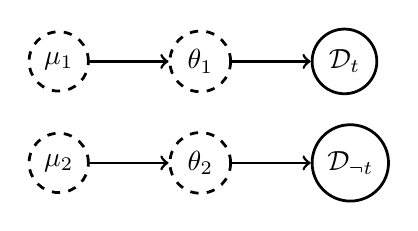
\begin{tikzpicture}
\node[circle, dashed, draw, line width=1pt] (D1) {$\mu_1$};
\node[circle, dashed, draw, below=0.5cm of D1, line width=1pt] (D2) {$\mu_2$};
\node[circle, dashed, draw, right=1cm of D1, line width=1pt] (mu1) {$\theta_1$};
\node[circle, dashed, draw, right=1cm of D2, line width=1pt] (mu2) {$\theta_2$};
\node[circle, draw, right=1cm of mu1, line width=1pt] (alpha) {$\mathcal{D}_t$};
\node[circle, draw, right=1cm of mu2, line width=1pt] (alpha1) {$\mathcal{D}_{\neg t}$};
\draw[->, line width=1pt] (D1.east) -- (mu1.west)  {};
\draw[->, line width=1pt] (D2.east) --  (mu2.west){};
\draw[->, line width=1pt] (mu1.east) --  (alpha.west){};
\draw[->, line width=1pt] (mu2.east) -- (alpha1.west) {};
\end{tikzpicture}
\end{document}